% Author: Rasmus Pank Roulund
\documentclass{standalone}
\usepackage{tikz}
\usetikzlibrary{shapes.geometric, arrows, positioning, calc, fit, arrows, decorations.pathreplacing}

\begin{document}

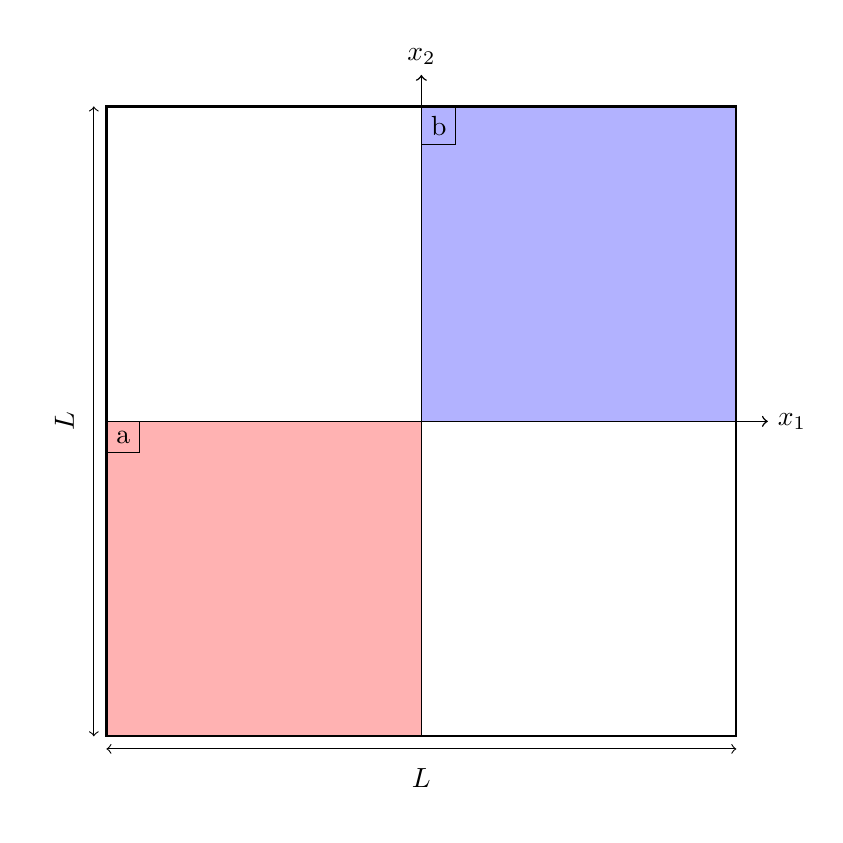
\begin{tikzpicture}[scale=4.0]


\def\outsize{1.25}
\draw[draw=none] (-\outsize,-\outsize) rectangle (\outsize,\outsize); 

\def\xd{0.25}

\draw[fill=blue!30!white] (0,0) rectangle (1.,1.);
\draw[fill=red!30!white] (-1.,-1.) rectangle (0.,0.);

\draw[line width=0.8pt] (-1.,-1.) rectangle (1.,1.);

\node[draw,anchor=north west] at (0,1) {b};
\node[draw,anchor=north west] at (-1,0) {a};

\draw[<->,line width=0.55pt] (0,1+0.1) node (yaxis) [above] {$x_2$}
        |- (1+0.1,0) node (xaxis) [right] {$x_1$};
        
\draw[<->] (-1.0,-1.04) --node[anchor=north,inner sep=7pt] {$L$} (1.,-1.04); 
\draw[<->] (-1.04,-1.) --node[rotate=90,anchor=south,inner sep=7pt] {$L$} (-1.04,1.); 



\end{tikzpicture}

\end{document}
